
Model Driven Development (MDD) is a top-down approach for the development of software systems. 
The main ideas of MDD were originally proposed by the Object Management Group (OMG)~\cite{mda}, as a set of guidelines for the structuring of specifications.
The technique advocates for the use of \textit{models} to specify a software system at different levels of abstraction (called \textit{viewpoints}):

\begin{trivlist}
\item \textbf{Computation Independent Models (CIM):} This level focusses on the
environment of the system, as well as on its business and requirement specifications. 
This viewpoint represents the software system at its highest level of abstraction. 
At this moment of the development, the structure and system processing details are still unknown or undetermined. 
 
\item \textbf{Platform Independent Models (PIM):} This level focusses on the system functionality, hiding the details of any particular platform. 
The specification defines those parts of the system that do not change from one platform to another. 

\item \textbf{Platform Specific Models (PSM):} This level focusses on the functionality, in the context of a particular implementation platform.
Models at this level combine the platform-independent view with the specific aspects of the platform to implement the system.  
\end{trivlist}

Besides the notion of model at each level of abstraction, MDD requires the use of \textit{model transformations} within and between levels.
Intra-level transformations are used to provide a unified representation of concepts of a given level.
Inter-level transformation implement a refinement process between levels.
Transformations may be automatic or semi-automatic.

MDD techniques has been successfully used for the development of hardware and software systems~\cite{MDDvariosAqui}. 
In particular, we are interested in the application of MDD to the design and implementation of web service applications.

Service oriented computing~\cite{Papazoglou2007} is at the origin of an evolution in the field of software development~\cite{??}. 
An important challenge of service oriented development is  to ensure the alignment between the requirements imposed by the business logic and the IT systems actually developed.
(Moreover, IT systems need to evolve according to the business needs.)
Thus, organizations are seeking for mechanisms to bridge the gap between the systems developed and business needs~\cite{bell}. 
The literature stresses the need for methodologies and techniques for service oriented analysis and design, claiming that they are the cornerstone  in the development of meaningful service based applications~\cite{5}.  
In this context, we argue that the convergence of model-driven software development, service orientation and better techniques for documenting and improving business processes are key to make real the idea of rapid, accurate development of software that serves, rather than dictates the needs of its users~\cite{watson}. 

In Service-Oriented Computing, pre-existing services are
combined to produce applications and provide the business logic. 
The selection of services is usually guided by the \textit{functional} requirements of the application being developed~\cite{1,2,decastro1,PapazoglouH06}. 
(Functional properties of a computer system are characterized by the effect produced by the system when given a defined input.)
Functional properties are not the only crucial aspect in the software development process. 
Other properties need to be addressed to fit in the application with its context.
These other aspects are called Non-Functional Properties.

Non-functional aspects of the services, often expressed as requirements and constraints in general purpose methodologies, are not usually considered from the beginning of the (service) software process.
Most methods consider them only after the application has been implemented, in order to ensure some level of reliability (e.g., data privacy, exception handling, atomicity, data persistence). 
This leads to service based applications that are partly specified and, thereby, partly compliant with the requirements of the application.
Ideally, non-functional requirements should be considered along with all the stages of the software development. 
The adoption of non-functional specifications from the early states of development
can help the developer to produce applications that are capable of dealing with
the application context.

In this work, we are interested in the extension of the \textit{Service Oriented Development Method} (SOD-M)~\cite{decastro1}, to support non-functional aspects, from the early stages of software development.
SOD-M is aligned with the MDD directives and proposes models, practices and techniques for the development of service-based applications.
SOD-M does not provide support for the specification of non-functional requirements, such as
security, reliability, and efficiency. 

The main goals of our work are:
\begin{trivlist}
\item \textit{(i)} To propose a methodology for supporting the construction of service-oriented applications, taking into account both functional and non-functional requirements;
\item \textit{(ii)} To improve the construction process by providing an abstract view of the application and ensure the conformance to its specification;
\item \textit{(iii)} To reduce the programming effort through the semi-automatic generation of  models for the application, to produce concrete implementations from high abstraction models;
\end{trivlist}

The rest of the paper is organized as follows. 
Section\dots

\COMMENT{
\subsection*{The rest of this section is just for draft\dots}

Non-functional properties of service oriented applications have been
addressed in academic works and standards~\cite{ws-co,ws-tra,wsci}.
Dealing with these kind of properties involves the use of specific technologies
in different layers of the SOC architecture, for instance during the description
of services APIs (such as WSDL\cite{wsdl} or REST~\cite{rest}) or to express
service coordinations (like WS-BPEL~\cite{bpel03}).

%Existing work addressing non-functional properties for service-oriented applications can be classified under four approaches:
%\begin{trivlist}
%\item[-] Those coming from the Business Process Domain and from the Web
%service standards that propose ad-hoc protocols. 
%Examples of these include the WS*-Family of the W3C\cite{ws-co,ws-tra,btp}.
%\item[-] Those adopting a classic middleware approach were non-functional
%properties are provided as middleware services, like the ones presented
%in~\cite{BeVaC00,RohmBSS02,NepalFGJKS05,Bonita}.
%\item[-] Those providing languages and enabling the specification of protocols
%used for expressing service
%compositions~\cite{LakhalKY05,LakhalKY05b,RouachedGABG06,FauvetDDB05}.
%\item[-] Those adopting separation of concerns,
%like~\cite{Milanovic06,Espinosa-OviedoVZC09,SchmelingCM11,PastranaPK11}.
%\end{trivlist}

Protocols and models implementing non-functional properties assume the existence of a global control of the artifacts implementing the application.
They also assume that each service exports its interface.
So, the challenge of supporting non-functional properties is related to
\textit{(i)} The specification of the business rules of the application; and 
\textit{(ii)} Dealing with the technical characteristics of the infrastructure where the application is executed.

%In this context, there is a need of 
%\textit{(i)} flexible protocols and models accepting a best effort approach for ensuring non-functional properties.
%\textit{(ii)} A methodology for specifying the application logic and its associated non-functional properties, starting at the early phases of the development process.
%
%In this work, we proppose to address the structured engineering of service-oriented applications in the presence of non-functional properties where: 
%\textit{(i)} The designer must make the diference between requirements that concern the application logic and the non-functional requirements;
%\textit{(ii)} General concepts must be provided to support the representation of  different non-functional requirements;
%\textit{(iii)} The non-functional requirements, specified in an abstract way, must provide enough information to be translated into the specification of technical aspects implementing concrete non-functional properties to be verified at runtime.










\[ \mathrm{Intro\ SAC} \]

Functional properties of a computer system are characterized by the effect produced by the system when given a defined input.
Functional properties are not the only crucial aspect in the software development process. 
Other properties need to be addressed to fit in the application with its context.
These other aspects are called Non-Functional Properties.

Non-Functional Requirements (NFRs) specify those properties that are not addressed by the functional  specification.
They are often called \textit{qualities} of the software system.
%They are also referred as ``constraints'', ``quality attributes'', ``quality goals'', ``quality of
%service requirements'' and ``non-behavioural requirements'' \cite{Stellman2005}.
Non-Functional Requirements may specify response time, security constraints or quality of the solution, among others.




Service-Oriented Computing~\cite{Papazoglou2007}, is a software development paradigm where pre-existing services are combined to produce more complex applications. 
%The selection of services is usually guided by the functional requirements of the application. 
%In this scenario, there exists the need to provide support for the specification of non-functional requirements, such as
%security, reliability, and efficiency. 
The development of service-based applications can benefit from the inclusion of NFRs to the software process from its early stages.
Failure to comply with this inclusion means that the final application is obtained from a partial specification, making the deployment a difficult task.
%Ideally, non-functional requirements
%would be considered along with all the stages of the software development. 
The adoption of non-functional specifications from the early states of development
can help the developer to produce applications that are capable of dealing with
their context.
Non-functional properties of service oriented applications have been
addressed in academic works and standards~\cite{ws-co,ws-tra,wsci}.
Different proposals~\cite{Babamir2010,AgarwalLS09,CholletL09,GutierrezRF10,XiaoCZBOLH08,JeongCL09,TsadimasNA12}
support non-functional requirements in the context of web service development. 

Most software development methods define software processes that use the notion of refinement.
Software process begins with the formulation of an abstract specification, which is successively refined to yield the implementation of the system.
Methods for the development of web service applications are no exception to this rule.
At least two levels of abstraction can be distinguished: a \textit{Business Level}, including the abstract specification, and a \textit{System Level}, including actual computer programs that implements the system.

In the case of web service applications we will distinguish two separate layers of the implementation.
The \textit{Composition Layer} is the upper layer of the implementation. 
It defines the workflow of the system, in terms of individual service calls.
The \textit{Service Layer} defines those services that are called by the composition.

\[ \mathrm{Original} \]
Service oriented computing is at the origin of an evolution in the field of software development. 
An important challenge of service oriented development is  to ensure the alignment between IT systems and the business logic.
%dealing thereby with the promise that IT systems can  evolve  according to the business needs. 
Thus, organizations are  seeking for mechanisms to deal with the gap between the systems developed and business needs \cite{bell}. The literature stresses the need for methodologies and techniques for service oriented analysis and design, claiming that they are the cornerstone  in the development of meaningful services' based applications \cite{5}.  In this context, some authors argue that the convergence of model-driven software development, service orientation and better techniques for documenting and improving business processes are the key to make real the idea of rapid, accurate development of software that serves, rather than dictates, software users' goals \cite{watson}. 

Service oriented development methodologies providing models, best practices, and reference architectures to build services' based applications mainly address  functional aspects \cite{1,2,decastro1,PapazoglouH06}.  Non-functional aspects concerning services' and application's "semantics", often expressed as requirements and constraints in general purpose methodologies, are not fully considered or they are added once the application has been implemented in order to ensure some level of reliability (e.g., data privacy, exception handling, atomicity, data persistence). This leads to services' based applications that are partially specified and that are thereby partially compliant with application requirements.

The objective of this work   is to model non-functional constraints and associate them to  services' based applications  early during the services' composition modeling phase. Therefore this paper presents $\pi$-SOD-M, a model-driven method  that extends the SOD-M  \cite{decastro1} for building reliable  services' based information systems (SIS). 
%SOD-M defines a process  starting with the  identification of business services through business modeling, and, by means of models' transformations it allows to obtain a services' composition model \cite{decastro1} and the executable code that implements it. 

Our work proposes to extend the SOD-M \cite{decastro1} method with  (i)  the notion of {\em A-Policy} \cite{Espinosa-Oviedo2011a} for representing non-functional constraints associated to services' based applications.  
%{\em A-policies} are used to express constraints which can be applied to all the services' composition  or to a particular service used for implementing it. They represent both systems' cross-cutting aspects (e.g., exception handling expressing what to do when a service is not available) and use constraints imposed by the services  (e.g., the fact that a service requires imposes an authentication protocol for executing a method). 
Our work  also (ii) defines the $\pi$-{\sc Pews}  meta-model \cite{Placido2010LTPD} providing guidelines for expressing the composition and the {\em A-policies}. Finally, our work (iii) defines model to model transformation rules for generating the $\pi$-{\sc Pews} model of a reliable services' composition starting from the extended services' composition model; and, model to text transformations for generating the corresponding implementation. As will be shown within our environment implementing these meta models and rules, one may represent both systems' cross-cutting aspects (e.g., exception handling for describing what to do when a service is not available, recovery, persistence aspects) and constraints associated to services, that must be respected for using them (e.g., the fact that a service requires an authentication protocol for executing a method). 

The remainder of the paper is organized as follows. Section \ref{sec:motivation} gives an overview of our approach. It describes a motivation example that integrates and synchronizes well-known social networks services namely Facebook, Twitter and, Spotify. Sections \ref{sec:piscm}, \ref{sec:pewsmetamodel}, and \ref{sec:mmrules} describe respectively the three key elements of our proposal, namelly the $\pi$-SCM and $\pi$-{\sc Pews} meta-models and the transformation rules that support the semi-automatic generation of reliable services' compositions.
%describes $\pi$-SOD-M method that enables the representation and association of {\em A-policies} to services' composition  thereby making them reliable. 
%
Section \ref{sec:implementation} describes implementation and validation issues.
Section \ref{sec:related} analyses related work concerning policy/contract based programming and, services' composition platforms. Section \ref{sec:conclusions} concludes the paper and discusses future work.

}

\bigskip
\textsc{The next two sections need to be relocated --Martin}
\bigskip

\section{SOD-M}\label{sec:sodm}
The Service-Oriented Development Method (SOD-M)~\cite{decastro1} is a MDD approach for service-based applications.
SOD-M provides a framework with models and standards to express functionalities of applications at a high-level of abstraction. 
SOD-M meta-models are organized into three levels: CIM (\textit{Computational Independent Models}), PIM (\textit{Platform Independent Models}) and PSM (\textit{Platform Specific Models}).

Two models are defined at the CIM level: \textit{value model} 
and \textit{BPMN model}. 
The PIM level models the entire structure of the application flow,
while, the PSM level provides transformations towards more specific platforms.
The PIM-level models are: \textit{use case}, \textit{extended use case}, \textit{service process} and
\textit{service composition}. The PSM level models are: \textit{web service interface}, \textit{extended composition service} and \textit{business logic}. 
These three levels have no support for describing non-functional requirements. 

The SOD-M approach includes transformations between models:
\textit{CIM-to-PIM, PIM-to-PIM} and \textit{PIM-to-PSM} transformations. Given
an abstract model at the CIM level, it is possible to apply transformations for
generating a model of the PSM level. In this context, it is necessary to
follow the process activities described by the methodology. 

SOD-M considers two points of view:
\textit{(i)} \textit{business}, focusing on the characteristics and requirements
of the organization, and \textit{(ii)} \textit{system requirements}, focusing on
features and processes to be implemented in order application requirements. In
this way, SOD-M aims to simplify the design of service-oriented applications, as
well as its implementation using current technologies.


\section{$\pi$SOD-M}\label{sec:pisodm}

%In this section we present $\pi$SOD-M, an MDD based methodology. 
$\pi$SOD-M provides an environment for building service compositions considering
their non-functional requirements. 
$\pi$SOD-M extends the SOD-M meta-models by adding
the concept of \textit{Policy}~\cite{Espinosa-Oviedo2011a}
to represent non-functional requirements.

\begin{figure}[h]
\centering
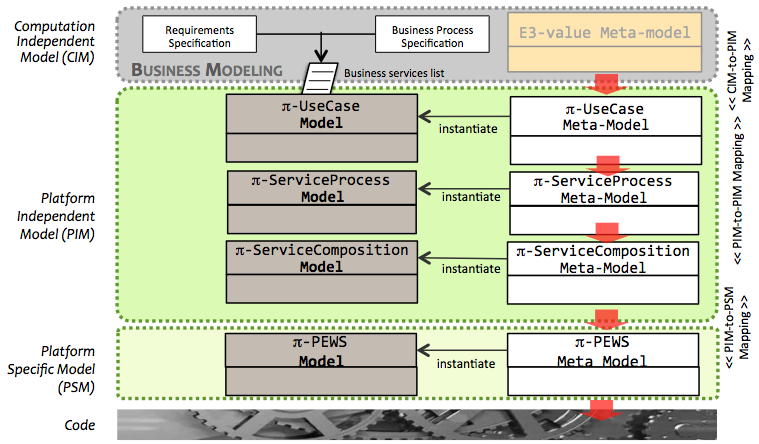
\includegraphics[width=1.0\textwidth]{figs/piSODM}
\caption{$\pi$SOD-M.}
\label{fig:piSOD-M}
\end{figure}

$\pi$SOD-M proposes the generation of a set of models at different abstraction levels, as
well as transformations between these models.
$\pi$SOD-M models represent both the functional aspects of the application as well as its non-functional constraints. 
Constraints are restrictions that must be verified during the execution of the application. 
An example of this is the requirement of the user's authentication for executing some system functions. 

Similarly to SOD-M, our approach targets the construction of service-oriented applications that implement business processes.
$\pi$SOD-M proposes a development process based on the definition of models
(instances of the meta-modes) and transformations between models.
There are two kinds of transformations:
Model-to-model transformations are used during the software process to refine the specification.
Model-to-text transformations are the last step of the process and generate code.

We extended SOD-M to include non-functional specifications.
Our method defines four meta-models: \textit{$\pi$-UseCase}, \textit{$\pi$-ServiceProcess}, \textit{$\pi$-ServiceCom\-po\-si\-tion} and \textit{$\pi$-PEWS}.
The former three are extensions of SOD-M meta-models and belong to the PIM level.
The \textit{$\pi$-PEWS} meta-model is a PSM (Figure~\ref{fig:piSOD-M}).

The \textit{$\pi$-UseCase} meta-model describes functional and non-functional requirements.
Non-functional requirements are defined as \textit{constraints} over processing and data. 
The \textit{$\pi$-ServiceProcess} meta-model defines the concept of \textit{service contract} to represent restrictions over data and actions that must be performed upon certain conditions. 
The \textit{$\pi$-ServiceProcess} meta-model gathers the constraints
described in the \textit{$\pi$-UseCase} model into contracts that are associated
with services. 
The \textit{$\pi$-ServiceComposition} meta-model provides the concept of \textit{Policy}
which put together contracts with similar non-functional requirements. 
For instance, security and privacy restrictions may be grouped into a security policy.
\textit{$\pi$-ServiceComposition} models can be refined into PSMs.

At the PSM level we have lower-level models that can be automatically translated into actual computer programs.
The \textit{$\pi$-PEWS} meta-model is the PSM adopted in this work.
\textit{$\pi$-PEWS} models are textual descriptions of service compositions that can be translated into PEWS code~\cite{BaCAM05,Placido2010LTPD}.
Although PEWS is our language of choice, other composition languages can be used as target.
This can be accomplished by defining: \textit{(i)} a model-to-model transformation, from a \textit{$\pi$-ServiceComposition} model to the corresponding PSM, and \textit{(ii)} a model-to-text transformation, from the this PSM to the composition language.

In the next section we develop an example, to serve as a proof-of-concept.
The example will show the actual notation used for models. 

